\section{Allgemeine Anforderungsbeschreibung}

\subsection{Ausgangssituation}

Die FastForward GmbH nutzt momentan einen IPv4-only-Anschluss und bekommt von ihrem Provider derzeit noch keinen IPv6-Anschluss. Da der IPv4-Adressraum im asiatischen Raum historisch bedingt nicht so groß ist wie beispielsweise der amerikanische, besteht gerade im asiatischen Raum ein erhöhter Bedarf an der zeitnahen Einführung von IPv6. Um die Kommunikation mit Kunden und Zulieferern in Fernost zu optimieren, die bereits IPv6 nutzen soll die eigene Nutzung von IPv6 getestet werden.

\subsection{Zielsetzung}

Es soll zunächst eine Testumgebung erstellt werden, die intern nur auf IPv6 basiert. Die Verbindung in das öffentliche Internet wird über einen Tunnel-Broker realisiert. In dieser Testumgebung sollen ein Web- und ein Mailserver betrieben werden, die öffentlich erreichbar sind. Optional ist darüber hinaus die Installation eines Active Directory und eines Domain Controllers.\section{Produkteinsatz}

\subsection{Anwendungsbereiche}
Der Anwendungsbereich unserer Lösung umfasst die gesamte Kommunikation, die innerhalb und aus der Testumgebung heraus über die Internetverbindung geführt wird. Die Testumgebung ist ausschließlich eine Machbarkeitsstudie, um auf den tatsächlichen Umstieg zu IPv6 vorbereitet zu sein.

\subsection{Zielgruppe}
Die Zielgruppe dieser Machbarkeitsstudie ist die IT-Abteilung des Unternehmens. Dabei soll ausgelotet werden, ob eine Umstellung des eigenen Netzwerkes auf IPv6 machbar ist. Damit ist die konkrete Zielgruppe das Projektteam, welches später die Umstellung durchführen soll.

\subsection{Betriebsbedingungen}

Die Umgebung soll 24 Stunden 7 Tage die Woche betrieben werden. Eine Beobachtung respektive Monitoring der Systeme ist kein Kriterium und findet entsprechend nur während den Arbeitszeiten an den Projekttagen statt.\\

\noindent{\bf Hardware}: Es stehen ein Router (Cisco 2800 Series), ein Switch (Cisco Catalyst 2960G Series) und ein no-name Server zur Verfügung. Als Test-Clients werden die eigenen Notebooks verwendet.\\
{\bf Orgware}: Es muss einen Aktiven Account bei SixXT, eine IPv4 Adresse des Providers und einen MX Record zur Verfügung gestellt werden.
\section{Produktfunktionen}

Im Rahmen des Projektes wird ein Segement des Netzwerkes der FastForward GmbH per IPv6 mit dem Internet verbunden. Damit Verbindungen zum IPv4-Internet möglich sind, wird ein Tunnel-Broker verwendet. Wir haben uns für die Verwendung von SixXS verwendet. Alternative Tunnel-Broker haben meist nur einen Standort. Beispielsweise IPv6Now in Australien oder 6frei in China. Der ähnlich breit aufgestellte Tunnel-Broker Hurricane Electric scheidet nur deswegen aus, weil SixXS mehr Protokolle unterstützt und damit für unsere Zwecke, die gesamte Kommunikation per IPv6 abzuwickeln besser geeignet ist.

Die Funktionen unseres Produktes umfassen die Abwicklung der Internetkommunikation per IPv6 und IPv4. Die interne Netzwerkkommunikation wird dabei ausschließlich per IPv6 realisiert. Damit die internen Clients nicht von außen erreichbar sind, werden zwei Subnetze realisiert, die durch die IPv6-Firewall getrennt werden.

\begin{itemize}
	\item Ausschließlich IPv6-basiertes Netzsegment
	\item Anbindung an das IPv6-Internet via Sixxs-Tunnel
	\item verschiedene Client-OS: Windows 10 und Ubuntu
	\item verschiedene Server-OS: Windows 2012R2 und Ubuntu 16.04
	\item IPv6-Firewall
\end{itemize}

\section{Projektumsetzung}

Die Umsetzung der Anforderungen wird mithilfe der bereitgestellten Hardware und des Tunnels über den Broker Sixxs realisiert. Da nur ein Server zur Verfügung steht, aber Server mit verschiedenen Betriebssystemen genutzt werden sollen, wird auf dem vorhandenen no-name Server ein Hypervisor auf Basis von Ubuntu 16.04 installiert. Über diesen werden zwei virtuelle Server eingerichtet. Der eine wird mit Windows 2012R2 betrieben und der andere ebenfalls mit Ubuntu 16.04. Auf letzterem werden sowohl Mailserver als auch Webserver realisiert. Sollte sich dieser Plan nicht umsetzen lassen, wird der no-name Server rein als Mail- und Webserver verwendet werden. Auf einem der Clients wird dann Windows 2012R2 installiert.

Mithilfe des Cisco Routers wird sowohl die Firewall als auch die Trennung des internen Netzwerkes in zwei Zonen realisiert. Bei den beiden Zonen handelt es sich um eine DMZ, in der sich der Mail- und Webserver befinden werden und um eine Trusted Zone, in der sich die Clients und der Windows-Server befinden werden. Die beiden Netzwerke erhalten jeweils ein eigenes IPv6-Subnetz und werden zudem durch VLANs voneinander getrennt. Die Firewall Regeln, Subnetze und VLANs werde im Netzwerkkonzept beschrieben.

\subsection{Skizzierung der Umsetzung}

\begin{wrapfigure}{r}{0.5\textwidth}
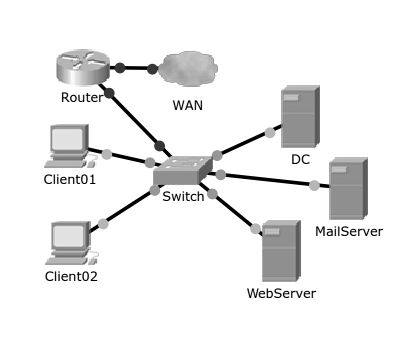
\includegraphics[scale=0.5]{../packettracer/8gruppe_netzaufbau.png}
\label{skizzierung-umsetzung}
\caption{Skizzierung der Umgebung}
\end{wrapfigure}

Die gezeigte Grafik beschreibt die von uns angestrebte, logische Umsetzung der Umgebung. Sowohl die Server als auch die Clients werden über den vorhandenen Cisco Switch miteinander verbunden. Der Switch wird per Router mit dem Internet (WAN) verbunden. Auf dem Router wird eine Firewall implementiert.







\section{Produktleistungen}

\noindent{\bf Muss-Kriterien}: Der Zugriff auf das öffentliche IPv6-Internet muss über eine IPv4-Adresse des Providers aus dem internen IPv6-Netzwerk möglich sein. Die interne Netzwerkkommunikation eines Web- und eines Mailservers muss dabei vollständig mit IPv6 realisiert werden. Clients müssen ebenfalls per IPv6 kommunizieren können. Die Testumgebung ist durch eine Firewall zu schützen. {\bf Wunschkriterien}: Optional kann ein Active Directory und ein Domain Controller eingerichtet werden. Clients soll es möglich sein, sich in der Domäne anzumelden. {\bf Abgrenzungskriterien}: Es handelt sich hierbei lediglich um eine Testumgebung. Sie ist nicht für den produktiven Einsatz geeignet.\section{Globale Testfälle}

Wir unterscheiden vier Kategorien von globalen Testfällen zur Bestimmung der Funktionalität. Die erste Kategorie umfasst die Funktionen des Mail- und Webserver und die zweite die Funktion des lokalen Netzwerkes. In der dritten Kategorie werden alle Tests zusammengefasst, die den Zugriff der Clients auf die Server betreffen. Abschließend wird in der vierten Kategorie getestet, ob das Netzwerksegment aus dem öffentlichen Internet erreichbar ist und ob die Services in der DMZ genutzt werden können.

\subsection{Mail- und Webserver}
\begin{itemize}
	\item[S01] Erreichbarkeit des Mailservers
	\item[S02] Erreichbarkeit des Webservers
	\item[S03] Der Webserver kann Mails senden und empfangen
\end{itemize}
\subsection{Lokales Netzwerk}
\begin{itemize}
	\item[I01] Kommunikation der Server und Clients per IPv6
	\item[I02] Trennung von Trusted Zone und DMZ per VLAN
	\item[I03] Kommunikation per IPv4 findet nicht statt
\end{itemize}
\subsection{Funktion der Clients}
\begin{itemize}
	\item[C01] Kommunikation der Clients mit IPv4-Server im Internet ist möglich
	\item[C02] Clients können über den Mailserver Emails senden und empfangen
	\item[C03] (optional) Clients können sich gegen die Windows Domäne authentifizieren
\end{itemize}
\subsection{Zugriff aus dem Internet}
\begin{itemize}
	\item[E01] Mail- und Webserver sind aus dem Internet erreichbar
	\item[E02] Clients sind aus dem Internet nicht erreichbar
	\item[E03] Firewall öffnet nur tatsächlich genutzte Ports
\end{itemize}

\section{Ergänzungen}

Wenn sich das Projekt erfolgreich realisieren lässt, sind für die Umsetzung in der Produktivumgebung noch einige Punkte zu beachten. Zum einen müssten alle nicht IPv6-fähigen Netzwerkgeräte ausgetauscht werden. Dasselbe gilt auch für alle Clients, wenn diese ihre IPv6-Verbindung nicht über einen internen IPv6-Tunnel realisieren. Als Alternative könnte die gesamte interne IPv4-Infrastruktur erhalten bleiben. Statt eines IPv6-zu-IPv4-Tunnels, wie in diesem Projekt verwendet, würde dann ein IPv4-zu-IPv6-Tunnel genutzt. Zum anderen ergibt sich für beide Umsetzungen ein Sicherheitsrisiko, da der jeweilige IPv4- oder IPv6-Netzwerkverkehr in beiden Fällen über einen zentralen Tunnel-Broker geroutet wird. Das bedeutet, dass in beiden Fällen ein eigener Tunnel-Broker betrieben werden.
